\section{Experiments}\label{sec:experiments}
Each claim is tested on the family~\eqref{eq:family} on a fixed grid of cells with hundreds of replicates and intervals on every cell metric.
Sections~\ref{sec:exp-c1}--\ref{sec:exp-c3} and Figures~\ref{fig:anatomy}--\ref{fig:crossover} report RMSE in outcome units ($\gate=2$, so ignoring interference gives RMSE near $1$); Table~\ref{tab:map} and Figure~\ref{fig:misspec} divide by $|\beta|+|\gamma|=2$, so \est{DM} is $0.5$.

\subsection{Variance follows leverage when the model is right}\label{sec:exp-c1}
With the correct model, independent noise and Bernoulli assignment (150 cells over $n\in[500,8000]$, $d\in[5,80]$, $p\in\{0.1,0.3,0.5\}$, $\sigma\in\{0.5,1\}$, 400 replicates; ER graphs), the standard deviation of $\that$ divided by $\sqrt{\sigma^2L/n}$ has median 1.01 and range 0.90--1.15, with no trend in any of the four factors; the Monte-Carlo noise of a standard deviation at this replicate count is about 3.5\%.
The ratio lies in $[0.94,1.09]$ in 32 cells on ER, SBM, BA and WS graphs ($n=2000$), and the iid interval covers 92--97\% everywhere.

The distance-two sandwich of Section~\ref{sec:anatomy} is accurate when $d^2/n$ is small (standard-error ratio 0.98 below 0.05), but its coverage falls from 0.94 at $d=5$ to 0.83, 0.60 and 0.23 at $d=20,40,80$ (medians), although the model is exact. A two-hop ball holds of order $d^2$ units, so the sandwich needs $n/d^2$ to be large.
Figure~\ref{fig:anatomy}c shows coverage rising with the number of independent two-hop balls $n/|B_2|$: at $d=40$ the sandwich covers 0.63 to 0.87 as $n$ grows from 2000 to 16000, while the iid interval stays at 0.93--0.97.
When only the assignment is redrawn (128 cells), the iid, HC3, cluster-robust and resampling standard errors are within 2\% of the true design standard deviation; under misspecification the failure is bias, not the variance estimator.

\begin{figure}[tb]
\centering
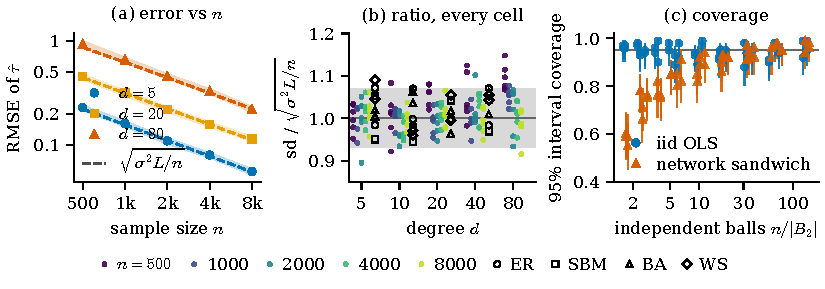
\includegraphics[width=\linewidth]{fig2_anatomy.pdf}
\caption{Variance of \est{REG-L} on a correctly specified linear response. (a) RMSE against $n$ at $d=5,20,80$ ($p=0.3$, $\sigma=1$, ER); dashed, $\sqrt{\sigma^2L/n}$; band, 95\% Monte-Carlo interval. (b) $\mathrm{sd}(\that)/\sqrt{\sigma^2L/n}$ in all 150 ER cells, coloured by $n$, and in the cells on four graph families at $n=2000$ (open); the grey band is the Monte-Carlo band around a ratio of one. (c) Coverage of the iid and distance-two sandwich 95\% intervals against the number of independent two-hop balls $n/|B_2|$, with Wilson 95\% bars.}
\label{fig:anatomy}
\end{figure}

\subsection{The bias floor is the projection bias and does not shrink with $n$}\label{sec:exp-c2}
Across a grid of 320 cells (ER, $n=2000$; $\kappa\in\{0,\tfrac14,\tfrac12,1\}$, three shapes, $p\in\{0.1,0.25,0.5,0.75\}$, $d\in\{5,10,20,50\}$, $\sigma\in\{0,0.5\}$, 200 replicates), the bias of \est{REG-L} equals the exact projection bias computed from the graph and design with independent seeds: correlation 0.9996, median absolute difference 0.006, maximum 0.033, no standardised difference above 3 (Figure~\ref{fig:bias}a). It grows with $\kappa$, $d$ and the asymmetry of $p$; the threshold shape keeps a bias of about 1.0 at $\kappa=1$, $p=\tfrac12$. For $\kappa>0$ the squared bias is a median 67\% of the mean squared error of \est{REG-L}, which beats \est{DM} in 98.6\% of those cells.
For $d=20$, $p=\tfrac14$ and a convex response, the bias of \est{REG-L} is $-0.47$ at every $n$ from 250 to 8000, against $-0.473$ predicted (Figure~\ref{fig:bias}b); the standard deviation falls as $n^{-1/2}$, so beyond $n=1000$ the error is bias.
More flexible features do not remove the floor at this corner distance. \est{REG-Q} has 3.7 times the standard deviation of \est{REG-L} at $n=8000$, and on the threshold response a bias of $+1.5$ against $-0.15$: the quadratic fit extrapolates in the wrong direction. \est{REG-O}, which has the true shape, is unbiased with 1.8 times the standard deviation.

\begin{figure}[tb]
\centering
\includegraphics[width=\linewidth]{fig3_projection_bias.pdf}
\caption{Bias of \est{REG-L} against the exact projection bias~\eqref{eq:bias}. (a) Measured against predicted in 320 cells (correlation 0.9996). (b) Bias against $n$ at $d=20$, $p=0.25$, $\sigma=0.5$ for \est{REG-L} on the convex and threshold responses, \est{REG-Q} and \est{REG-O}; dashed lines are the predictions, and \est{DM} sits at $-1$.}
\label{fig:bias}
\end{figure}

\subsection{Who regression loses to}\label{sec:exp-c3}
\begin{figure}[tb]
\centering
\includegraphics[width=\linewidth]{fig4_crossover.pdf}
\caption{RMSE of $\that$ against mean degree $d$ on ER graphs ($n\approx2000$, Bernoulli, $\sigma=0.5$, 300 replicates; $\gate=2$). The exact variance of full-exposure \est{HT} is computed from the pair formula; all other estimators are evaluated on the same draws. Left to right: linear response with $p=\tfrac12$; convex response with $p=\tfrac15$; threshold response with $p=\tfrac12$.}
\label{fig:crossover}
\end{figure}
Full-exposure \est{HT} is unbiased, and its exact RMSE rises from 0.28 at $d=2$ to 0.97, 12, $1.8\times10^3$ and $2.6\times10^9$ at $d=5,10,20,50$ ($p=\tfrac12$; Figure~\ref{fig:crossover}), while \est{REG-L} stays between 0.04 and 0.16 in the linear cells. Across all 100 (response, $p$, $d$) combinations, $d$ from 2 to 50, \est{REG-L} has the lower RMSE, so a crossover with exact \est{HT} exists only at degrees of about one to two.
The relevant competitors also trade bias for variance: the Hájek estimator, which falls back to the arm mean when no unit is exposed and so approaches \est{DM} (RMSE 1.0) once $d\gtrsim15$--20, and its relaxed versions.
Over the 100 combinations, with a paired bootstrap over replicates (Appendix, Table~\ref{tab:wins}), \est{REG-L} beats \est{DM} in 96 and loses in 4; beats the practical Hájek estimator in 83 (11 losses) and the Hájek estimator with a relaxation $\delta$ chosen by a declared rule in 84 (13 losses); with the best $\delta$ in each cell, which uses the truth, it wins in 77 and loses in 17.
Every loss to the declared relaxed Hájek is in the threshold response at $p=\tfrac12$ (for $\kappa=1$ at all ten degrees). There \est{REG-L} has RMSE 0.09 ($d=2$), 0.83 (10) and 1.61 (50), against 0.07, 0.49 and 1.00 for the practical Hájek estimator; for $d\ge15$ it is worse than ignoring interference (1.08--1.61 against 1.00).
Regression, a line, beats relaxed exposure, a step, and \est{DM}, a constant, unless the response is step-like with the step near the middle of the exposure range.

\subsection{One summary of the degree organises the error across graphs}\label{sec:exp-c4}
Section~\ref{sec:anatomy} gives the distances~\eqref{eq:z} for a regular graph. On a graph with heterogeneous degrees the question is which summary of the degrees to use. We test $d$ as the harmonic and as the arithmetic mean on ER, SBM, BA and WS graphs ($n=2000$, $d$ from 5 to 80), on Stanford3 and on ego-Facebook (thinned to vary $d$), over $p\in\{0.1,0.25,0.5\}$ (261 cells, 200 replicates).
\begin{figure}[tb]
\centering
\includegraphics[width=\linewidth]{fig5_collapse.pdf}
\caption{Collapse of the error in the corner distances. (a) $\mathrm{sd}(\that)\sqrt n/\sigma$ against $Z_0+Z_1=\sqrt{d/(p(1-p))}$ with $d$ the harmonic mean degree (filled) or the arithmetic mean (open), on a correctly specified linear response; 87 graph settings. (b) Bias normalised by the outcome scale, measured against predicted by a cubic in $(\log Z_1,\log Z_0)$ fitted on five graph families and evaluated on the sixth; filled, threshold response; open, concave response. Stanford3 plateaus off the diagonal. (c) Held-out $R^2$ by predictor. Points in (a) and (b) are single fitted cells and (c) is one held-out fit per predictor, so none has an interval.}
\label{fig:collapse}
\end{figure}
For the variance the identity $\mathrm{sd}(\that)\sqrt n/\sigma=Z_0+Z_1$ has no fitted parameter. With the harmonic mean degree its $R^2$ is 0.97, the Spearman correlation 0.99 and the median absolute log ratio 5.7\%, against a Monte-Carlo error of about 5\% (Figure~\ref{fig:collapse}a). It is 0.98--0.99 on ER, SBM, BA and WS and 0.82--0.85 on the two real graphs. With the arithmetic mean it is 0.61 ($-5.9$ on Stanford3, where the observed standard deviation is 0.54 of the prediction): the pooled exposure variance is $p(1-p)\,\overline{1/d_i}$, the harmonic mean.
For the bias, we fit a cubic in $(\log Z_1,\log Z_0)$ on five families and predict the sixth (threshold response with $\kappa=\tfrac12$ and concave response with $\kappa=1$). The held-out $R^2$ is 0.97 and 0.90 with the harmonic mean and 0.77 and 0.75 with the arithmetic mean; the worst family is Stanford3, whose bias plateaus.
Two qualifications bound this. First, $(Z_0,Z_1)$ is a reparametrisation of $(d,p)$, and a polynomial in $(\log d_{\mathrm{hm}},p)$ predicts as well (held-out $R^2$ 0.97 and 0.90): what is carried is the harmonic mean, not a new variable. Second, one coordinate is not enough ($Z_1$ alone has held-out $R^2$ 0.27 and 0.62, $Z_0$ alone 0.48 and 0.04): the bias depends on the pair, the variance on $Z_0+Z_1$.

\subsection{Where regression holds and fails}\label{sec:exp-c5}
\begin{table}[tb]
\caption{RMSE$/(|\beta|+|\gamma|)$ by mechanism and estimator, median / worst over six graphs (ER, SBM, BA, WS at $n=2000$, $d=20$; ego-Facebook thinned to $n=4039$; Stanford3 thinned to $n=11586$), $p=\tfrac12$, $\sigma=0.5$, 100 replicates; \est{DM} is $0.50$ by construction. Hájek$_{.25}$ is the relaxed Hájek estimator with $\delta=0.25$. Intervals are in Tables~\ref{tab:cmedian} and~\ref{tab:cworst}. Bold: the lowest non-oracle median and any entry whose interval overlaps it; grey: the oracle \est{REG-O}, which knows the response form and bounds what any regression can do. $^\dagger$\est{GCN} was not run on Stanford3 (median and worst over five graphs). The exact \est{HT} has RMSE of $10^{33}$ or more here and is omitted.}
\label{tab:map}
\centering
\input{../tables/tab1_method_mechanism.tex}
\end{table}
Table~\ref{tab:map} crosses ten mechanisms with the estimators.
\emph{Where \est{REG-L} is right it is far better than the alternatives.} On linear, concave, convex and heterogeneous-direct responses its median error is 0.05, against 0.50 for \est{DM} and 0.23--0.27 for the relaxed Hájek estimator, and its worst graph is 0.06--0.07, real graphs included. Its measured bias equals the exact projection bias in all 60 cells (correlation 0.9998), so Section~\ref{sec:exp-c2} carries to mechanisms it was not tuned on.
\emph{Flexibility does not remove the floor.} \est{REG-Q} is within noise of \est{REG-L} in 42 of 60 cells. \est{REG-G}, which adds the two-hop exposure, an interaction and log degree, is worse in 43, by a factor of 2.6--3 on one-hop mechanisms through variance. Boosted trees and the graph network carry a bias of about 0.2 on a linear response, because they do not extrapolate to $g=1$; they win only where the corner lies on a plateau the sample sees (trees on the threshold: 0.12 against 0.56) or the model class contains the omitted term (graph network, two-hop: 0.15--0.16 against 0.25).
\emph{The map has regions where regression fails.} (i) The saturating threshold at $0.5$ is the one mechanism where \est{REG-L} is worse than \est{DM} on the synthetic graphs (0.53--0.64 against 0.50); on ego-Facebook and Stanford3 it gives 0.21 and 0.17. There 23--24\% of the units have degree at most five, which spreads $g$ over $[0,1]$ and puts both plateaus of the step inside the data (mass .13--.15 against .01 on ER, SBM and WS); fitted on those units alone the bias is 0.10--0.14. The relaxed Hájek estimator and trees (0.10--0.12) are better, but cannot be chosen without knowing the response. (ii) A two-hop component of weight $\tfrac12$ raises the error from 0.05 to 0.25 on every graph except WS, almost entirely as bias; only models that contain the two-hop exposure come down (0.14--0.16). (iii) A response proportional to degree gives a bias of $-0.37$ on ego-Facebook and Stanford3 (error 0.38) and at most 0.06 on ER, SBM and WS; the count-feature variant is right there (0.01--0.05) and wrong elsewhere. (iv) Heterogeneous indirect effects cost 0.28 and 0.33 on the two real graphs against at most 0.10 elsewhere, even for the oracle.

\emph{An error in the observed graph} costs bias $-q\gamma$ when a fraction $q$ of the edges is wrong: the error rises from 0.048 to 0.074, 0.14 and 0.27 at $q=0.1,0.25,0.5$, still below \est{DM}, and no richer feature set helps because the exposure is not measured (Appendix~\ref{app:results}).

\subsection{Design levers}\label{sec:exp-c7}
The design can put the corner into the data, at a price: clusters that match communities cut the \est{REG-L} error to 0.20--0.83 of its Bernoulli value but gain little without communities, and a staggered rollout is unbiased at the cost of repeated measurements and no carry-over (Appendix~\ref{app:results}).
